% Activate the following line by filling in the right side. If for example the name of the root file is Main.tex, write
% "...root = Main.tex" if the chapter file is in the same directory, and "...root = ../Main.tex" if the chapter is in a subdirectory.
 
%!TEX root =  mainMastersProject.tex

\chapter[Simple Spatial Simulations]{A Simple Robbery - Spatial Simulations and their Bayesian Networks}

Three experiments: 1) getting the bayesian networks with disturbances (). 2) testing the effect of a simulation parameter change on the BN (how different does it become. 3) investigating the effect of hidden information/private knowledge on the network.
Summary:

 The problem is that in the previous chapter, we have established that we have a method to convert a simple, forward chaining simulation, to a collection of data, which then in turn can be used to create a Bayesian Network, that represents the situation in the simulation relatively well (some problems none-withstanding, accuracy and RMS error are generally ok even in increments that people might plausibly be able to estimate ~ intervals of 0.33/0.25-ish). However, this was totally 100\% determined by deterministic forward chaining rules. The real world does not run on deterministic forward chaining rules (as far as we know). At least, we are spatially situated, which means that there are probabilities that will arise out of interactions between agents and their environment. These probabilities are not `set' in the same ways as the probabilities are set in the previous chapter, they arise organically from interactions: eg: an agent has to be located at a door to break in, an agent can be seen by a camera only in some locations of the simulation. We do not know these probabilities a-priori (although we can probably calculate them, I don't know).
 
New idea: We create spatially situated simulations that are more complex, and see if they work the same way/are as accurate \& rms as the previous. Then we will also use these simple spatial simulations to test two hypotheses about 1) the effect of private knowledge and 2) the effect of parameters.


\section{Experiment 1: Generating BNs with disturbances}
\subsection{Introduction}
Here I talk about the robbery example with the evidence.
Also model reference class explicitly just for fun here.



\subsection{Methods}

Same as before. 

\subsection{Results}


See Figure~\ref{laptopAcc}

\begin{figure}[h!]
\begin{center}
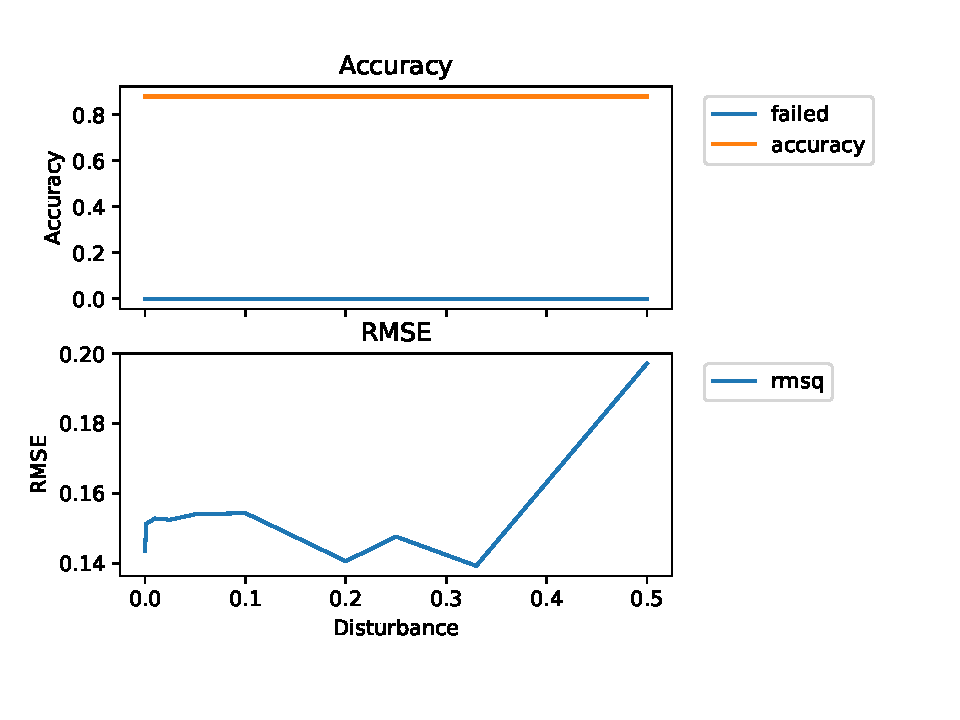
\includegraphics[]{../experiments/StolenLaptop/plots/performance_StolenLaptop.pdf}
\caption{Accuracy (100\% to 0\%) and Root Mean Square error (1 - 0) for rounding to different intervals in stolenLaptop network and simulation}
\label{laptopAcc}
\end{center}
\end{figure}

Overall pretty accurate.


\subsection{Discussion}





\section{Experiment 2: Investigating the evidence strength depending on parameters of the network.}


\subsection{Introduction}
A funny thing is that this simulation we can test how the evidence strength is dependent on certain parameters in the network. For a simple example, see the radius of camera vision. If we have the Reporter ``agent seen near house''/"agent spotted by camera", and by that we mean, that if the agent is visible in the camera placed near the house, then the range of vision of the camera becomes relevant for the investigation. If the camera is super good and can see the agent even when he's not near the house, then the effect of being-seen-on-camera should decrease: it becomes less relevant that the agent was seen by the camera, because they usually are. On the other hand, if the camera is pointed only at the door, then being seen by the camera is relevant, the agent is only by the door when he's trying to break in. Below you see a plot of camera vision range vs effect on posterior when the node is turned on (given the same structure of the BN).

\subsection{Methods}
I changed the parameter of vision of the camera for the simulation between 1 and 15, for the rest the simulation was the exact same. I didn't apply any disturbances to the network.

\subsection{Results}



\subsection{Discussion}
We see here, that the name of the variable is actually incorrect. It shouldn't be called "agent seen near house", because the reporter is not actually reporting that the agent is near the house - instead it is reporting whether the agent is within the vision of the camera. So properly it should be called "agent is seen in camera", or we can rewrite the reporter to measure whether the agent is actually near the house. 

But, this means that the BN is responsive to the effect of relevance in the real world. If a piece of information is less relevant, it will reflect that. But you have to know exactly what you're measuring.

How natural language names relate to reporters, is actually a really difficult question that I will address in more detail later.

How would a judge/lawyer interpret this?


\section{Experiment 3: Investigating the effect of private knowledge}

\subsection{Introduction}

\subsection{Method}
Drop column Private knowledge and evidence for it, see the effect on the posterior. See the effect on the disturbances.


\subsection{Results}
New network.
New accuracy and RMS plots.

\subsection{Discussion}

How would a judge/lawyer interpret this?


\section{Take aways from the three experiments}

Simulating works, accuracy and RMS fine.

We run into problems when we use words like `near' in our node names. We're lucky that we know what we mean (because our reporter forces us to make this explicit). We do not just ground the probabilities in our network, but we actually also ground our random variables - we have a measure of exactly what events we are interested in, and which we aren't.

We are in trouble with private knowledge, dropping this column from our table (which means that we don't know it) when we make our BN, we're drastically reducing our uh. Accuracy, and increasing our RMS. This implies that we do seem to need a full picture of everything that's happening, otherwise our BN will be kind of shit, and be less accurate :(.

Hence, for a simulation to work we 1) need to know exactly what it is that we're measuring since evidence strength depends on it \footnote{explain this more}, and 2) private information is necessary to create the BN because it influences fleeing behaviour. If we don't have this information our BN will be shit.


